\documentclass[twoside]{book}

% Packages required by doxygen
\usepackage{fixltx2e}
\usepackage{calc}
\usepackage{doxygen}
\usepackage[export]{adjustbox} % also loads graphicx
\usepackage{graphicx}
\usepackage[utf8]{inputenc}
\usepackage{makeidx}
\usepackage{multicol}
\usepackage{multirow}
\PassOptionsToPackage{warn}{textcomp}
\usepackage{textcomp}
\usepackage[nointegrals]{wasysym}
\usepackage[table]{xcolor}

% Font selection
\usepackage[T1]{fontenc}
\usepackage[scaled=.90]{helvet}
\usepackage{courier}
\usepackage{amssymb}
\usepackage{sectsty}
\renewcommand{\familydefault}{\sfdefault}
\allsectionsfont{%
  \fontseries{bc}\selectfont%
  \color{darkgray}%
}
\renewcommand{\DoxyLabelFont}{%
  \fontseries{bc}\selectfont%
  \color{darkgray}%
}
\newcommand{\+}{\discretionary{\mbox{\scriptsize$\hookleftarrow$}}{}{}}

% Page & text layout
\usepackage{geometry}
\geometry{%
  a4paper,%
  top=2.5cm,%
  bottom=2.5cm,%
  left=2.5cm,%
  right=2.5cm%
}
\tolerance=750
\hfuzz=15pt
\hbadness=750
\setlength{\emergencystretch}{15pt}
\setlength{\parindent}{0cm}
\setlength{\parskip}{3ex plus 2ex minus 2ex}
\makeatletter
\renewcommand{\paragraph}{%
  \@startsection{paragraph}{4}{0ex}{-1.0ex}{1.0ex}{%
    \normalfont\normalsize\bfseries\SS@parafont%
  }%
}
\renewcommand{\subparagraph}{%
  \@startsection{subparagraph}{5}{0ex}{-1.0ex}{1.0ex}{%
    \normalfont\normalsize\bfseries\SS@subparafont%
  }%
}
\makeatother

% Headers & footers
\usepackage{fancyhdr}
\pagestyle{fancyplain}
\fancyhead[LE]{\fancyplain{}{\bfseries\thepage}}
\fancyhead[CE]{\fancyplain{}{}}
\fancyhead[RE]{\fancyplain{}{\bfseries\leftmark}}
\fancyhead[LO]{\fancyplain{}{\bfseries\rightmark}}
\fancyhead[CO]{\fancyplain{}{}}
\fancyhead[RO]{\fancyplain{}{\bfseries\thepage}}
\fancyfoot[LE]{\fancyplain{}{}}
\fancyfoot[CE]{\fancyplain{}{}}
\fancyfoot[RE]{\fancyplain{}{\bfseries\scriptsize Generated by Doxygen }}
\fancyfoot[LO]{\fancyplain{}{\bfseries\scriptsize Generated by Doxygen }}
\fancyfoot[CO]{\fancyplain{}{}}
\fancyfoot[RO]{\fancyplain{}{}}
\renewcommand{\footrulewidth}{0.4pt}
\renewcommand{\chaptermark}[1]{%
  \markboth{#1}{}%
}
\renewcommand{\sectionmark}[1]{%
  \markright{\thesection\ #1}%
}

% Indices & bibliography
\usepackage{natbib}
\usepackage[titles]{tocloft}
\setcounter{tocdepth}{3}
\setcounter{secnumdepth}{5}
\makeindex

% Hyperlinks (required, but should be loaded last)
\usepackage{ifpdf}
\ifpdf
  \usepackage[pdftex,pagebackref=true]{hyperref}
\else
  \usepackage[ps2pdf,pagebackref=true]{hyperref}
\fi
\hypersetup{%
  colorlinks=true,%
  linkcolor=blue,%
  citecolor=blue,%
  unicode%
}

% Custom commands
\newcommand{\clearemptydoublepage}{%
  \newpage{\pagestyle{empty}\cleardoublepage}%
}

\usepackage{caption}
\captionsetup{labelsep=space,justification=centering,font={bf},singlelinecheck=off,skip=4pt,position=top}

%===== C O N T E N T S =====

\begin{document}

% Titlepage & ToC
\hypersetup{pageanchor=false,
             bookmarksnumbered=true,
             pdfencoding=unicode
            }
\pagenumbering{alph}
\begin{titlepage}
\vspace*{7cm}
\begin{center}%
{\Large Stack \\[1ex]\large 3.\+0 }\\
\vspace*{1cm}
{\large Generated by Doxygen 1.8.13}\\
\end{center}
\end{titlepage}
\clearemptydoublepage
\pagenumbering{roman}
\tableofcontents
\clearemptydoublepage
\pagenumbering{arabic}
\hypersetup{pageanchor=true}

%--- Begin generated contents ---
\chapter{Main Page}
\label{index}\hypertarget{index}{}Implements a stack class

See files\+:
\begin{DoxyItemize}
\item \hyperlink{stack_8h}{stack.\+h}
\item \hyperlink{stack_8cpp}{stack.\+cpp}
\end{DoxyItemize}

\begin{DoxyVersion}{Version}
1.\+0
\end{DoxyVersion}
\begin{DoxyAuthor}{Author}
ShJ 
\end{DoxyAuthor}
\begin{DoxyDate}{Date}
2017 
\end{DoxyDate}

\chapter{Namespace Index}
\section{Namespace List}
Here is a list of all documented namespaces with brief descriptions\+:\begin{DoxyCompactList}
\item\contentsline{section}{\hyperlink{namespacestk}{stk} }{\pageref{namespacestk}}{}
\end{DoxyCompactList}

\chapter{Class Index}
\section{Class List}
Here are the classes, structs, unions and interfaces with brief descriptions\+:\begin{DoxyCompactList}
\item\contentsline{section}{\hyperlink{classatom_1_1array__t}{atom\+::array\+\_\+t$<$ Tp, max\+\_\+size\+\_\+ $>$} }{\pageref{classatom_1_1array__t}}{}
\item\contentsline{section}{\hyperlink{classatom_1_1bad_alloc}{atom\+::bad\+Alloc} \\*Exception about problems with allocate of the memory }{\pageref{classatom_1_1bad_alloc}}{}
\item\contentsline{section}{\hyperlink{classatom_1_1error}{atom\+::error} \\*Abstract class which is template for all exceptions }{\pageref{classatom_1_1error}}{}
\item\contentsline{section}{\hyperlink{classatom_1_1invalid_argument}{atom\+::invalid\+Argument} \\*Exception about problems with arguments in functions }{\pageref{classatom_1_1invalid_argument}}{}
\item\contentsline{section}{\hyperlink{classatom_1_1invalid_object}{atom\+::invalid\+Object} \\*Exception about problems with object different classes }{\pageref{classatom_1_1invalid_object}}{}
\item\contentsline{section}{\hyperlink{classatom_1_1other_error}{atom\+::other\+Error} \\*Undefine here exceptions }{\pageref{classatom_1_1other_error}}{}
\item\contentsline{section}{\hyperlink{classatom_1_1out_of_range}{atom\+::out\+Of\+Range} \\*Exception about problems connected with borders }{\pageref{classatom_1_1out_of_range}}{}
\item\contentsline{section}{\hyperlink{struct_p_o_i_s_o_n}{P\+O\+I\+S\+O\+N$<$ Tp $>$} \\*Poison constant for any elements }{\pageref{struct_p_o_i_s_o_n}}{}
\item\contentsline{section}{\hyperlink{struct_p_o_i_s_o_n_3_01char_01_4}{P\+O\+I\+S\+O\+N$<$ char $>$} }{\pageref{struct_p_o_i_s_o_n_3_01char_01_4}}{}
\item\contentsline{section}{\hyperlink{struct_p_o_i_s_o_n_3_01double_01_4}{P\+O\+I\+S\+O\+N$<$ double $>$} }{\pageref{struct_p_o_i_s_o_n_3_01double_01_4}}{}
\item\contentsline{section}{\hyperlink{struct_p_o_i_s_o_n_3_01float_01_4}{P\+O\+I\+S\+O\+N$<$ float $>$} }{\pageref{struct_p_o_i_s_o_n_3_01float_01_4}}{}
\item\contentsline{section}{\hyperlink{struct_p_o_i_s_o_n_3_01int_01_4}{P\+O\+I\+S\+O\+N$<$ int $>$} }{\pageref{struct_p_o_i_s_o_n_3_01int_01_4}}{}
\item\contentsline{section}{\hyperlink{struct_p_o_i_s_o_n_3_01long_01long_01_4}{P\+O\+I\+S\+O\+N$<$ long long $>$} }{\pageref{struct_p_o_i_s_o_n_3_01long_01long_01_4}}{}
\item\contentsline{section}{\hyperlink{struct_p_o_i_s_o_n_3_01short_01_4}{P\+O\+I\+S\+O\+N$<$ short $>$} }{\pageref{struct_p_o_i_s_o_n_3_01short_01_4}}{}
\item\contentsline{section}{\hyperlink{struct_p_o_i_s_o_n_3_01unsigned_01char_01_4}{P\+O\+I\+S\+O\+N$<$ unsigned char $>$} }{\pageref{struct_p_o_i_s_o_n_3_01unsigned_01char_01_4}}{}
\item\contentsline{section}{\hyperlink{struct_p_o_i_s_o_n_3_01unsigned_01int_01_4}{P\+O\+I\+S\+O\+N$<$ unsigned int $>$} }{\pageref{struct_p_o_i_s_o_n_3_01unsigned_01int_01_4}}{}
\item\contentsline{section}{\hyperlink{struct_p_o_i_s_o_n_3_01unsigned_01long_01long_01_4}{P\+O\+I\+S\+O\+N$<$ unsigned long long $>$} }{\pageref{struct_p_o_i_s_o_n_3_01unsigned_01long_01long_01_4}}{}
\item\contentsline{section}{\hyperlink{struct_p_o_i_s_o_n_3_01unsigned_01short_01_4}{P\+O\+I\+S\+O\+N$<$ unsigned short $>$} }{\pageref{struct_p_o_i_s_o_n_3_01unsigned_01short_01_4}}{}
\item\contentsline{section}{\hyperlink{classatom_1_1stack__t}{atom\+::stack\+\_\+t$<$ Tp, Container $>$} }{\pageref{classatom_1_1stack__t}}{}
\item\contentsline{section}{\hyperlink{classatom_1_1vector__t}{atom\+::vector\+\_\+t$<$ Tp $>$} }{\pageref{classatom_1_1vector__t}}{}
\end{DoxyCompactList}

\chapter{File Index}
\section{File List}
Here is a list of all documented files with brief descriptions\+:\begin{DoxyCompactList}
\item\contentsline{section}{D\+:/\+Git\+Hub/\+Techno\+Atom/src/\hyperlink{debug__tools_8h}{debug\+\_\+tools.\+h} }{\pageref{debug__tools_8h}}{}
\item\contentsline{section}{D\+:/\+Git\+Hub/\+Techno\+Atom/src/\hyperlink{exceptions_8h}{exceptions.\+h} }{\pageref{exceptions_8h}}{}
\item\contentsline{section}{D\+:/\+Git\+Hub/\+Techno\+Atom/src/array/\hyperlink{array_8h}{array.\+h} }{\pageref{array_8h}}{}
\item\contentsline{section}{D\+:/\+Git\+Hub/\+Techno\+Atom/src/array/implement/{\bfseries array.\+hpp} }{\pageref{array_8hpp}}{}
\item\contentsline{section}{D\+:/\+Git\+Hub/\+Techno\+Atom/src/stack/\hyperlink{stack_8h}{stack.\+h} }{\pageref{stack_8h}}{}
\item\contentsline{section}{D\+:/\+Git\+Hub/\+Techno\+Atom/src/stack/implement/{\bfseries stack.\+hpp} }{\pageref{stack_8hpp}}{}
\item\contentsline{section}{D\+:/\+Git\+Hub/\+Techno\+Atom/src/vector/\hyperlink{vector_8h}{vector.\+h} }{\pageref{vector_8h}}{}
\item\contentsline{section}{D\+:/\+Git\+Hub/\+Techno\+Atom/src/vector/implement/{\bfseries vector.\+hpp} }{\pageref{vector_8hpp}}{}
\end{DoxyCompactList}

\chapter{Namespace Documentation}
\hypertarget{namespacestk}{}\section{stk Namespace Reference}
\label{namespacestk}\index{stk@{stk}}
\subsection*{Classes}
\begin{DoxyCompactItemize}
\item 
class \hyperlink{classstk_1_1stack__t}{stack\+\_\+t}
\end{DoxyCompactItemize}


\subsection{Detailed Description}
There the stack class describes 
\chapter{Class Documentation}
\hypertarget{classstk_1_1stack__t}{}\section{stk\+:\+:stack\+\_\+t$<$ Tp, stack\+\_\+size $>$ Class Template Reference}
\label{classstk_1_1stack__t}\index{stk\+::stack\+\_\+t$<$ Tp, stack\+\_\+size $>$@{stk\+::stack\+\_\+t$<$ Tp, stack\+\_\+size $>$}}


{\ttfamily \#include $<$stack.\+h$>$}



Collaboration diagram for stk\+:\+:stack\+\_\+t$<$ Tp, stack\+\_\+size $>$\+:
\nopagebreak
\begin{figure}[H]
\begin{center}
\leavevmode
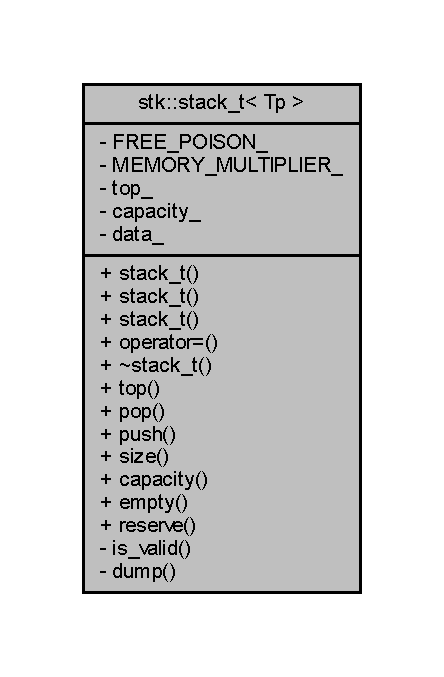
\includegraphics[width=198pt]{classstk_1_1stack__t__coll__graph}
\end{center}
\end{figure}
\subsection*{Public Types}
\begin{DoxyCompactItemize}
\item 
\mbox{\Hypertarget{classstk_1_1stack__t_a05d1586fa8257268f0c1ade7ffc4588e}\label{classstk_1_1stack__t_a05d1586fa8257268f0c1ade7ffc4588e}} 
using \hyperlink{classstk_1_1stack__t_a05d1586fa8257268f0c1ade7ffc4588e}{value\+\_\+type} = Tp
\begin{DoxyCompactList}\small\item\em Element type. \end{DoxyCompactList}\item 
\mbox{\Hypertarget{classstk_1_1stack__t_a27d586bc06e0faf30a2a980cd8ffd125}\label{classstk_1_1stack__t_a27d586bc06e0faf30a2a980cd8ffd125}} 
using \hyperlink{classstk_1_1stack__t_a27d586bc06e0faf30a2a980cd8ffd125}{const\+\_\+value\+\_\+type} = const Tp
\begin{DoxyCompactList}\small\item\em Const element type. \end{DoxyCompactList}\item 
\mbox{\Hypertarget{classstk_1_1stack__t_ade199c494a8e4455f76cc04faf138ed8}\label{classstk_1_1stack__t_ade199c494a8e4455f76cc04faf138ed8}} 
using \hyperlink{classstk_1_1stack__t_ade199c494a8e4455f76cc04faf138ed8}{size\+\_\+type} = std\+::size\+\_\+t
\begin{DoxyCompactList}\small\item\em Size type. \end{DoxyCompactList}\end{DoxyCompactItemize}
\subsection*{Public Member Functions}
\begin{DoxyCompactItemize}
\item 
\hyperlink{classstk_1_1stack__t_ab7605ffb3efbfdaf23c1411dba8076d7}{stack\+\_\+t} ()
\item 
\mbox{\Hypertarget{classstk_1_1stack__t_a27abcc49011f8cd22cd92395655f8ca4}\label{classstk_1_1stack__t_a27abcc49011f8cd22cd92395655f8ca4}} 
\hyperlink{classstk_1_1stack__t_a27abcc49011f8cd22cd92395655f8ca4}{stack\+\_\+t} (const \hyperlink{classstk_1_1stack__t}{stack\+\_\+t} \&)=default
\begin{DoxyCompactList}\small\item\em Default the copy constructor. \end{DoxyCompactList}\item 
\mbox{\Hypertarget{classstk_1_1stack__t_a680884feaecd4cb19ea890893c583fdb}\label{classstk_1_1stack__t_a680884feaecd4cb19ea890893c583fdb}} 
\hyperlink{classstk_1_1stack__t}{stack\+\_\+t} \& \hyperlink{classstk_1_1stack__t_a680884feaecd4cb19ea890893c583fdb}{operator=} (const \hyperlink{classstk_1_1stack__t}{stack\+\_\+t} \&)=default
\begin{DoxyCompactList}\small\item\em Default the assignment operator. \end{DoxyCompactList}\item 
\mbox{\Hypertarget{classstk_1_1stack__t_acd6dfd6efc2edad5c9bd8f126c415a69}\label{classstk_1_1stack__t_acd6dfd6efc2edad5c9bd8f126c415a69}} 
\hyperlink{classstk_1_1stack__t_acd6dfd6efc2edad5c9bd8f126c415a69}{$\sim$stack\+\_\+t} ()=default
\begin{DoxyCompactList}\small\item\em Default destructor. \end{DoxyCompactList}\item 
\hyperlink{classstk_1_1stack__t_a05d1586fa8257268f0c1ade7ffc4588e}{value\+\_\+type} \hyperlink{classstk_1_1stack__t_a120f150bc90f8ccf0c0ca8396bda7c65}{top} () const
\item 
void \hyperlink{classstk_1_1stack__t_a5be99b150a46b8456643cbc40bcefca8}{pop} ()
\item 
void \hyperlink{classstk_1_1stack__t_aad7638faa441f17e91ba9a8f5663be4c}{push} (\hyperlink{classstk_1_1stack__t_a27d586bc06e0faf30a2a980cd8ffd125}{const\+\_\+value\+\_\+type} \&x)
\item 
\hyperlink{classstk_1_1stack__t_ade199c494a8e4455f76cc04faf138ed8}{size\+\_\+type} \hyperlink{classstk_1_1stack__t_a50dbd2e6626510af69ba1f38882ca1b5}{size} () const
\item 
bool \hyperlink{classstk_1_1stack__t_adb144d5de96aeeed6dee8d902158f1a6}{empty} () const
\end{DoxyCompactItemize}
\subsection*{Private Member Functions}
\begin{DoxyCompactItemize}
\item 
bool \hyperlink{classstk_1_1stack__t_a6c1813c8dc347f0cc9ab94a6e120d743}{is\+\_\+valid} () const
\item 
void \hyperlink{classstk_1_1stack__t_ac6b1f910422f3402f4ffcc8d496d0273}{dump} () const
\end{DoxyCompactItemize}
\subsection*{Private Attributes}
\begin{DoxyCompactItemize}
\item 
\mbox{\Hypertarget{classstk_1_1stack__t_a34489e147dc7052c6ee4eaa70c31c009}\label{classstk_1_1stack__t_a34489e147dc7052c6ee4eaa70c31c009}} 
\hyperlink{classstk_1_1stack__t_a27d586bc06e0faf30a2a980cd8ffd125}{const\+\_\+value\+\_\+type} \hyperlink{classstk_1_1stack__t_a34489e147dc7052c6ee4eaa70c31c009}{F\+R\+E\+E\+\_\+\+P\+O\+I\+S\+O\+N\+\_\+} = static\+\_\+cast$<$\hyperlink{classstk_1_1stack__t_a27d586bc06e0faf30a2a980cd8ffd125}{const\+\_\+value\+\_\+type}$>$(0)
\begin{DoxyCompactList}\small\item\em Constant for mark the empty fields. \end{DoxyCompactList}\item 
\mbox{\Hypertarget{classstk_1_1stack__t_a740287c74a7e188220ef94e4dbd5a3ea}\label{classstk_1_1stack__t_a740287c74a7e188220ef94e4dbd5a3ea}} 
\hyperlink{classstk_1_1stack__t_a05d1586fa8257268f0c1ade7ffc4588e}{value\+\_\+type} \hyperlink{classstk_1_1stack__t_a740287c74a7e188220ef94e4dbd5a3ea}{data\+\_\+} \mbox{[}stack\+\_\+size\mbox{]}
\begin{DoxyCompactList}\small\item\em Stack base on array. \end{DoxyCompactList}\item 
\mbox{\Hypertarget{classstk_1_1stack__t_a9c23414b1fa07a11c14f2abb029ee676}\label{classstk_1_1stack__t_a9c23414b1fa07a11c14f2abb029ee676}} 
\hyperlink{classstk_1_1stack__t_ade199c494a8e4455f76cc04faf138ed8}{size\+\_\+type} \hyperlink{classstk_1_1stack__t_a9c23414b1fa07a11c14f2abb029ee676}{top\+\_\+}
\begin{DoxyCompactList}\small\item\em Pointer on the top item of the stack. \end{DoxyCompactList}\end{DoxyCompactItemize}


\subsection{Detailed Description}
\subsubsection*{template$<$typename Tp, std\+::size\+\_\+t stack\+\_\+size = 10$>$\newline
class stk\+::stack\+\_\+t$<$ Tp, stack\+\_\+size $>$}


\begin{DoxyTemplParams}{Template Parameters}
{\em Tp} & the type of the value in the stack \\
\hline
{\em stack\+\_\+size} & the capacity of the stack (the default value is 10) \\
\hline
\end{DoxyTemplParams}


\subsection{Constructor \& Destructor Documentation}
\mbox{\Hypertarget{classstk_1_1stack__t_ab7605ffb3efbfdaf23c1411dba8076d7}\label{classstk_1_1stack__t_ab7605ffb3efbfdaf23c1411dba8076d7}} 
\index{stk\+::stack\+\_\+t@{stk\+::stack\+\_\+t}!stack\+\_\+t@{stack\+\_\+t}}
\index{stack\+\_\+t@{stack\+\_\+t}!stk\+::stack\+\_\+t@{stk\+::stack\+\_\+t}}
\subsubsection{\texorpdfstring{stack\+\_\+t()}{stack\_t()}}
{\footnotesize\ttfamily template$<$typename Tp , std\+::size\+\_\+t stack\+\_\+size = 10$>$ \\
\hyperlink{classstk_1_1stack__t}{stk\+::stack\+\_\+t}$<$ Tp, stack\+\_\+size $>$\+::\hyperlink{classstk_1_1stack__t}{stack\+\_\+t} (\begin{DoxyParamCaption}{ }\end{DoxyParamCaption})\hspace{0.3cm}{\ttfamily [inline]}}

Default constructor Fill all elements F\+R\+E\+E\+\_\+\+P\+O\+I\+S\+O\+N\+\_\+ 

\subsection{Member Function Documentation}
\mbox{\Hypertarget{classstk_1_1stack__t_ac6b1f910422f3402f4ffcc8d496d0273}\label{classstk_1_1stack__t_ac6b1f910422f3402f4ffcc8d496d0273}} 
\index{stk\+::stack\+\_\+t@{stk\+::stack\+\_\+t}!dump@{dump}}
\index{dump@{dump}!stk\+::stack\+\_\+t@{stk\+::stack\+\_\+t}}
\subsubsection{\texorpdfstring{dump()}{dump()}}
{\footnotesize\ttfamily template$<$typename Tp , std\+::size\+\_\+t stack\+\_\+size$>$ \\
void \hyperlink{classstk_1_1stack__t}{stk\+::stack\+\_\+t}$<$ Tp, stack\+\_\+size $>$\+::dump (\begin{DoxyParamCaption}{ }\end{DoxyParamCaption}) const\hspace{0.3cm}{\ttfamily [private]}}

Dumper Create file \char`\"{}\+\_\+\+\_\+stack\+\_\+dump.\+txt\char`\"{} where is information about stack\textquotesingle{}s status \mbox{\Hypertarget{classstk_1_1stack__t_adb144d5de96aeeed6dee8d902158f1a6}\label{classstk_1_1stack__t_adb144d5de96aeeed6dee8d902158f1a6}} 
\index{stk\+::stack\+\_\+t@{stk\+::stack\+\_\+t}!empty@{empty}}
\index{empty@{empty}!stk\+::stack\+\_\+t@{stk\+::stack\+\_\+t}}
\subsubsection{\texorpdfstring{empty()}{empty()}}
{\footnotesize\ttfamily template$<$typename Tp , std\+::size\+\_\+t stack\+\_\+size = 10$>$ \\
bool \hyperlink{classstk_1_1stack__t}{stk\+::stack\+\_\+t}$<$ Tp, stack\+\_\+size $>$\+::empty (\begin{DoxyParamCaption}{ }\end{DoxyParamCaption}) const\hspace{0.3cm}{\ttfamily [inline]}}

Checks the emptiness of the stack \begin{DoxyReturn}{Returns}
true if stack is empty, otherwise false 
\end{DoxyReturn}
\mbox{\Hypertarget{classstk_1_1stack__t_a6c1813c8dc347f0cc9ab94a6e120d743}\label{classstk_1_1stack__t_a6c1813c8dc347f0cc9ab94a6e120d743}} 
\index{stk\+::stack\+\_\+t@{stk\+::stack\+\_\+t}!is\+\_\+valid@{is\+\_\+valid}}
\index{is\+\_\+valid@{is\+\_\+valid}!stk\+::stack\+\_\+t@{stk\+::stack\+\_\+t}}
\subsubsection{\texorpdfstring{is\+\_\+valid()}{is\_valid()}}
{\footnotesize\ttfamily template$<$typename Tp , std\+::size\+\_\+t stack\+\_\+size$>$ \\
bool \hyperlink{classstk_1_1stack__t}{stk\+::stack\+\_\+t}$<$ Tp, stack\+\_\+size $>$\+::is\+\_\+valid (\begin{DoxyParamCaption}{ }\end{DoxyParamCaption}) const\hspace{0.3cm}{\ttfamily [private]}}

Silent verifier \begin{DoxyReturn}{Returns}
True if stack is valid else return false 
\end{DoxyReturn}
\mbox{\Hypertarget{classstk_1_1stack__t_a5be99b150a46b8456643cbc40bcefca8}\label{classstk_1_1stack__t_a5be99b150a46b8456643cbc40bcefca8}} 
\index{stk\+::stack\+\_\+t@{stk\+::stack\+\_\+t}!pop@{pop}}
\index{pop@{pop}!stk\+::stack\+\_\+t@{stk\+::stack\+\_\+t}}
\subsubsection{\texorpdfstring{pop()}{pop()}}
{\footnotesize\ttfamily template$<$typename Tp , std\+::size\+\_\+t stack\+\_\+size$>$ \\
void \hyperlink{classstk_1_1stack__t}{stk\+::stack\+\_\+t}$<$ Tp, stack\+\_\+size $>$\+::pop (\begin{DoxyParamCaption}{ }\end{DoxyParamCaption})}

Delete the item from the stack 
\begin{DoxyExceptions}{Exceptions}
{\em std\+::exception} & From \hyperlink{stack_8h_a4ad7af85cae2910ffcf6bfbcb8278886}{A\+S\+S\+E\+R\+T\+\_\+\+V\+A\+L\+I\+D()} when stack is not valid \\
\hline
{\em std\+::out\+\_\+of\+\_\+range} & When stack is empty \\
\hline
\end{DoxyExceptions}
\mbox{\Hypertarget{classstk_1_1stack__t_aad7638faa441f17e91ba9a8f5663be4c}\label{classstk_1_1stack__t_aad7638faa441f17e91ba9a8f5663be4c}} 
\index{stk\+::stack\+\_\+t@{stk\+::stack\+\_\+t}!push@{push}}
\index{push@{push}!stk\+::stack\+\_\+t@{stk\+::stack\+\_\+t}}
\subsubsection{\texorpdfstring{push()}{push()}}
{\footnotesize\ttfamily template$<$typename Tp , std\+::size\+\_\+t stack\+\_\+size$>$ \\
void \hyperlink{classstk_1_1stack__t}{stk\+::stack\+\_\+t}$<$ Tp, stack\+\_\+size $>$\+::push (\begin{DoxyParamCaption}\item[{\hyperlink{classstk_1_1stack__t_a27d586bc06e0faf30a2a980cd8ffd125}{const\+\_\+value\+\_\+type} \&}]{x }\end{DoxyParamCaption})}

Append new item in the stack 
\begin{DoxyExceptions}{Exceptions}
{\em std\+::exception} & From \hyperlink{stack_8h_a4ad7af85cae2910ffcf6bfbcb8278886}{A\+S\+S\+E\+R\+T\+\_\+\+V\+A\+L\+I\+D()} when stack is not valid \\
\hline
{\em std\+::out\+\_\+of\+\_\+range} & When the stack is full \\
\hline
\end{DoxyExceptions}
\mbox{\Hypertarget{classstk_1_1stack__t_a50dbd2e6626510af69ba1f38882ca1b5}\label{classstk_1_1stack__t_a50dbd2e6626510af69ba1f38882ca1b5}} 
\index{stk\+::stack\+\_\+t@{stk\+::stack\+\_\+t}!size@{size}}
\index{size@{size}!stk\+::stack\+\_\+t@{stk\+::stack\+\_\+t}}
\subsubsection{\texorpdfstring{size()}{size()}}
{\footnotesize\ttfamily template$<$typename Tp , std\+::size\+\_\+t stack\+\_\+size = 10$>$ \\
\hyperlink{classstk_1_1stack__t_ade199c494a8e4455f76cc04faf138ed8}{size\+\_\+type} \hyperlink{classstk_1_1stack__t}{stk\+::stack\+\_\+t}$<$ Tp, stack\+\_\+size $>$\+::size (\begin{DoxyParamCaption}{ }\end{DoxyParamCaption}) const\hspace{0.3cm}{\ttfamily [inline]}}

Currently size of the stack \begin{DoxyReturn}{Returns}
Count of the item in the stack 
\end{DoxyReturn}
\mbox{\Hypertarget{classstk_1_1stack__t_a120f150bc90f8ccf0c0ca8396bda7c65}\label{classstk_1_1stack__t_a120f150bc90f8ccf0c0ca8396bda7c65}} 
\index{stk\+::stack\+\_\+t@{stk\+::stack\+\_\+t}!top@{top}}
\index{top@{top}!stk\+::stack\+\_\+t@{stk\+::stack\+\_\+t}}
\subsubsection{\texorpdfstring{top()}{top()}}
{\footnotesize\ttfamily template$<$typename Tp , std\+::size\+\_\+t stack\+\_\+size = 10$>$ \\
\hyperlink{classstk_1_1stack__t_a05d1586fa8257268f0c1ade7ffc4588e}{value\+\_\+type} \hyperlink{classstk_1_1stack__t}{stk\+::stack\+\_\+t}$<$ Tp, stack\+\_\+size $>$\+::top (\begin{DoxyParamCaption}{ }\end{DoxyParamCaption}) const\hspace{0.3cm}{\ttfamily [inline]}}

Get the item from the stack 
\begin{DoxyExceptions}{Exceptions}
{\em std\+::exception} & From \hyperlink{stack_8h_a4ad7af85cae2910ffcf6bfbcb8278886}{A\+S\+S\+E\+R\+T\+\_\+\+V\+A\+L\+I\+D()} when stack is not valid \\
\hline
\end{DoxyExceptions}
\begin{DoxyReturn}{Returns}
the top item from the stack 
\end{DoxyReturn}


The documentation for this class was generated from the following files\+:\begin{DoxyCompactItemize}
\item 
D\+:/\+Git\+Hub/\+Techno\+Atom/stack/\hyperlink{stack_8h}{stack.\+h}\item 
D\+:/\+Git\+Hub/\+Techno\+Atom/stack/\hyperlink{stack_8cpp}{stack.\+cpp}\end{DoxyCompactItemize}

\chapter{File Documentation}
\hypertarget{stack_8h}{}\section{D\+:/\+Git\+Hub/\+Techno\+Atom/stack/stack.h File Reference}
\label{stack_8h}\index{D\+:/\+Git\+Hub/\+Techno\+Atom/stack/stack.\+h@{D\+:/\+Git\+Hub/\+Techno\+Atom/stack/stack.\+h}}
{\ttfamily \#include $<$stdexcept$>$}\newline
{\ttfamily \#include $<$cassert$>$}\newline
{\ttfamily \#include $<$fstream$>$}\newline
{\ttfamily \#include $<$ctime$>$}\newline
\subsection*{Classes}
\begin{DoxyCompactItemize}
\item 
class \hyperlink{classstk_1_1stack__t}{stk\+::stack\+\_\+t$<$ Tp, stack\+\_\+size $>$}
\end{DoxyCompactItemize}
\subsection*{Namespaces}
\begin{DoxyCompactItemize}
\item 
 \hyperlink{namespacestk}{stk}
\begin{DoxyCompactList}\small\item\em There the stack class describes. \end{DoxyCompactList}\end{DoxyCompactItemize}
\subsection*{Macros}
\begin{DoxyCompactItemize}
\item 
\mbox{\Hypertarget{stack_8h_aec2864553519b450501f110ca0c3e3b7}\label{stack_8h_aec2864553519b450501f110ca0c3e3b7}} 
\#define {\bfseries S\+T\+A\+C\+K\+\_\+H}
\item 
\#define \hyperlink{stack_8h_a4ad7af85cae2910ffcf6bfbcb8278886}{A\+S\+S\+E\+R\+T\+\_\+\+V\+A\+L\+ID}()
\end{DoxyCompactItemize}


\subsection{Macro Definition Documentation}
\mbox{\Hypertarget{stack_8h_a4ad7af85cae2910ffcf6bfbcb8278886}\label{stack_8h_a4ad7af85cae2910ffcf6bfbcb8278886}} 
\index{stack.\+h@{stack.\+h}!A\+S\+S\+E\+R\+T\+\_\+\+V\+A\+L\+ID@{A\+S\+S\+E\+R\+T\+\_\+\+V\+A\+L\+ID}}
\index{A\+S\+S\+E\+R\+T\+\_\+\+V\+A\+L\+ID@{A\+S\+S\+E\+R\+T\+\_\+\+V\+A\+L\+ID}!stack.\+h@{stack.\+h}}
\subsubsection{\texorpdfstring{A\+S\+S\+E\+R\+T\+\_\+\+V\+A\+L\+ID}{ASSERT\_VALID}}
{\footnotesize\ttfamily \#define A\+S\+S\+E\+R\+T\+\_\+\+V\+A\+L\+ID(\begin{DoxyParamCaption}{ }\end{DoxyParamCaption})}

{\bfseries Value\+:}
\begin{DoxyCode}
\{\(\backslash\)
    if (!is\_valid()) \{\(\backslash\)
        dump();\(\backslash\)
        assert(!\textcolor{stringliteral}{"Stack is good"});\(\backslash\)
        throw std::exception();\(\backslash\)
    \}\(\backslash\)
\}
\end{DoxyCode}
Macro to test object integrity 
\begin{DoxyExceptions}{Exceptions}
{\em std\+::exception} & Stack is not valid \\
\hline
\end{DoxyExceptions}

%--- End generated contents ---

% Index
\backmatter
\newpage
\phantomsection
\clearemptydoublepage
\addcontentsline{toc}{chapter}{Index}
\printindex

\end{document}
